\documentclass{book}
\usepackage[utf8]{inputenc}
\usepackage{amssymb}
\usepackage{blindtext}
\usepackage[english]{babel}
\usepackage{graphicx}
\usepackage{wrapfig}
\usepackage[english]{babel}
\usepackage{algorithm}
\usepackage{algpseudocode}
\usepackage{amsthm}
\newtheorem{definition}{Definition}[section]
\newcommand{\norm}[1]{\left\lVert#1\right\rVert}
\newtheorem{theorem}{Theorem}[section]
\newtheorem{corollary}{Corollary}[theorem]
\newtheorem*{Importante}{\textbf{Importante}}
\newtheorem{lemma}[theorem]{Lemma}
\usepackage{amsmath}
\usepackage{tikz}
\usetikzlibrary{shapes.geometric, arrows}
\usepackage{geometry}
\geometry{a4paper, top=2cm, bottom=2cm, left=1.5cm, right=1.5cm}
\usepackage{imakeidx}
\usepackage[T1]{fontenc}
\makeindex[columns=3, title=Alphabetical Index, intoc]
\title{Computer and Network Security}
\author{Lorenzo Rossi}
\graphicspath{{Images/}}
\begin{document}
\theoremstyle{definition}
\maketitle
\tableofcontents
\newpage
\part{Third Midterm}
\chapter{Secret Sharing}
\section{Trivial Secret Sharing}\mbox{}\\
Supponiamo di avere un segreto e vogliamo dividerne la conoscenza in due persone (dette shareholders)\@.
Inoltre, vogliamo si viene a conoscenza del segreto se e solo se entrambe le parti rivelano la loro porzione di segreto.
\begin{figure*}[h]
    \centering
    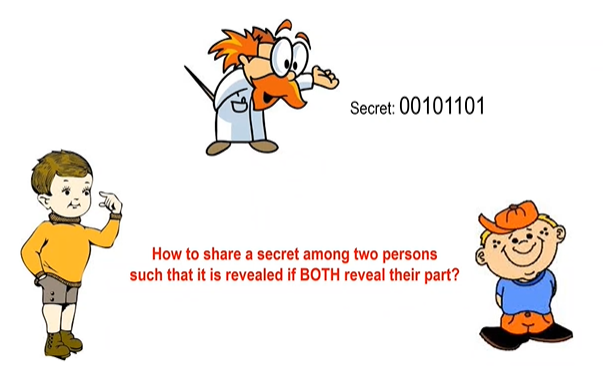
\includegraphics[scale=0.5]{2021-12-26-17-16-35.png}% chktex 8
\end{figure*}
Chi fornisce il segreto viene detto \textbf{dealer}, mentre chi riceve le porzioni del segreto sono detti \textbf{share}\@.\newline
Nel caso in cui avessimo diviso il segreto in parti uguali, è una pessima idea poiché per indovinare il segreto abbiamo \(\frac{1}{2^{N_{bit}}}\) probabilità di indovinare la password ed ora, avendo diviso il segreto in parti uguali, abbiamo una probabilità molto maggiore \(\frac{1}{2^{\frac{N_{bit}}{2}}}\) \@.
\subsection{XOR Secret Sharing}
Possiamo fare di meglio:\begin{enumerate}
    \item Prendi il segreto i.e.0010.1101;
    \item Genera una sequenza casuale \textbf{key} i.e.1011.0100;
    \item XOR il segreto e il valore casuale \textbf{one time pad} i.e.1001.1001;\newline
          Fino ad ora abbiamo applicato un \emph{Vernam cipher}\@.
    \item Diamo ad uno share la sequenza casuale, mentre ad un altro diamo il valore dello XOR;\@
    \item L'unione fra gli share da la chiave\@.
\end{enumerate}
\begin{Importante}
    Il conoscere la chiave, cioè il valore casuale, non mi da alcuna informazione riguardante la chiave\@.\newline Lo stesso discorso vale per il valore dello XOR poiché, come dimostrato nel \textbf{perfect secrecy}, l'operatore di XOR tra una stringa pseudocasuale e un valore casuale non da informazioni su quale sia la password\@.\newline
    Questi due aspetti rappresentano un requisito di sicurezza\@.
\end{Importante}
\newpage
\subsection{Modular Secret Sharing}
Un altro possibile schema è quello di utilizzare le somme modulari:\begin{enumerate}
    \item Prendi il segreto S in bit, trasformalo in digit i.e.0010.1101\(rightarrow\)45;
    \item Genera \(RAND\mod{N}\) i.e.\(RAND\mod{256} \rightarrow  180\);
    \item Esegui \(S-RAND\mod{N}\) i.e. \(S-RAND\mod{256}\rightarrow  121\);
\end{enumerate}
\begin{Importante}
    Questo schema è equivalente ad One Time Pad poiché abbiamo sommato un numero pseudocasuale con un numero casuare (in modulo)\@. In altre parole, la probabilità di indovinare S conoscendo il valore casuale o il valore della somma è uguale alla probabilità di indovinare senza sapere nulla\@.
\end{Importante}
Questo metodo è più facile da implementare per essere condiviso con N shareholders\@. In particolare, genero 3 quantità truly random ed effettua la differenza tra il segreto e queste 3 quantità modulo N\@.
Nel caso un attacker, riuscisse ad ottenere un numero sufficiente di share non può comunque ottenere la password, ma al più la differenza tra il segreto e le shares non prese\@.\newline Da qui è possibile definire il concetto di \textbf{perfect secrecy}: un avversario, conoscendo n-1 shares deve ancora possedere la probabilità di indovinare il segreto pari a quella di indovinare il segreto da zero\@.
\subsection{Shamir Secret Sharing}
Fino ad ora abbiamo costruito uno schema detto (n,n) secret sharing scheme in cui il primo parametro è il numero delle persone necessarie a rilevare il segreto e il secondo parametor è il numero di parti:\@il segreto viene rilevato solo se tutte le n parti forniscono il segreto\@.\newline
Un altro schema è \textbf(t,n) secret sharing scheme:\@il segreto è rilevato quando qualsiasi t delle n parti fornisce il segreto\@. Questo secondo problema è molto più complicato del trivial secret sharing\@.
\subsubsection{Idea:\@Schema (2,n)}
Il problema è quello di modellare uno schema per cui, conoscendo 2 degli n shareholders, posso ricostruire il segreto\@. Questo problema è riconducibile a quello di conoscere quanti punti sono necessari per definire una linea:\@ovviamente 2\@.
\begin{figure*}[h]
    \centering
    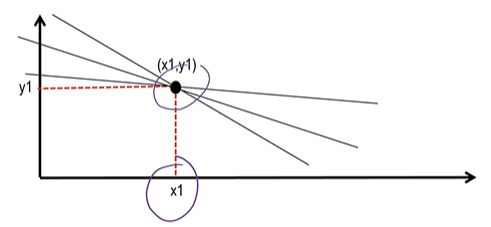
\includegraphics[scale=0.5]{2021-12-26-18-33-00.png}% chktex 8
\end{figure*}
Infatti conoscendo un solo punto (shares) ho infinite rette passanti per quel punto e quindi è impossibile ricondurci al segreto;\@tuttavia, conoscendo 2 punti (shares), tra essi passa solamente una sola retta e conseguentemente posso conoscere il segreto\@. Abbiamo comunque mantenuto la proprietà di poter avere un numero maggiore di 2 per ottenere il segreto, ma al minimo sono 2\@.
\subsubsection{Procedura: Generalizzazione schema\((2,n)\)}
\begin{itemize}
    \item \textbf{Dealer:} costruisce la linea:
          \begin{enumerate}
              \item Coefficiente a:\@scelto casualemnte;
              \item Segreto S:\@noto;
                    \begin{equation*}
                        \centering
                        y=S+ax
                    \end{equation*}
          \end{enumerate}
          Per esempio: \(a=15\quad S=39\)
    \item Distribuisci le shares ai n partecipanti scegliendo casualmente il valore \(x_{i}\) da introdurre nell'equazione della retta:
          \begin{itemize}
              \item Shareholder 1: \(x_{1}=1\rightarrow share=(1,54)\);
              \item Shareholder 2: \(x_{2}=2\rightarrow share=(2,69)\);
              \item Shareholder 3: \(x_{3}=3\rightarrow share=(3,84)\);
              \item \dots
          \end{itemize}
\end{itemize}
\begin{Importante}
    La y viene calcolata in base alla funzione della retta;\@tuttavia, i punti degli shareholder sono mantenuti con (x,y) e il valore delle \(x_{i}\) possono essere noti a priori a patto che la y sia nascosta\@.
\end{Importante}
\subsubsection{Procedura: Ricostruzione}
\begin{itemize}
    \item Ricezione di due shares:\(P_{i}=(x_{i},y_{i})\quad P_{j}=(x_{j},y_{j})\);
\end{itemize}
SONO ARRIVATO A CNS 24: 0:44:11
\end{document}